%DO NOT MESS AROUND WITH THE CODE ON THIS PAGE UNLESS YOU %REALLY KNOW WHAT YOU ARE DOING
\chapter{Mechanical Components of the Machine} \label{Mechanical Components of the Machine}
\section{CAD Model} \label{CAD Model}

\begin{figure}[H]
  \centering
    \begin{minipage}{0.40\textwidth}
    \centering
      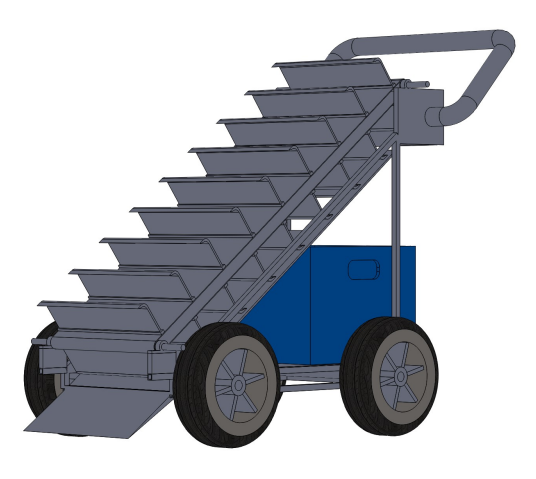
\includegraphics[width=1\textwidth]{cad 2.PNG}

    \end{minipage}
    \begin{minipage}{0.40\textwidth}
    \centering
      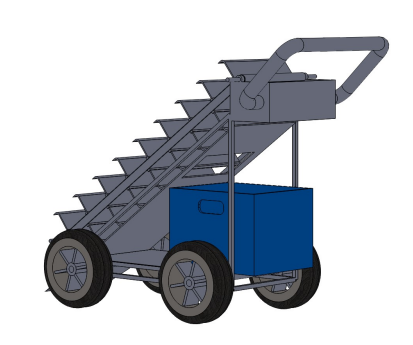
\includegraphics[width=1\textwidth]{cad 1.PNG}
     \end{minipage}
    \caption{Final 3D CAD Model}
\end{figure}

\section{Main Frame} \label{Main Frame}
It is the supporting structure of the machine on which the other various components are mounted. It should be strong enough to withstand the dead weight of all the components as well as the forces which will be transmitted during operation.
\begin{figure}[h!]
\center
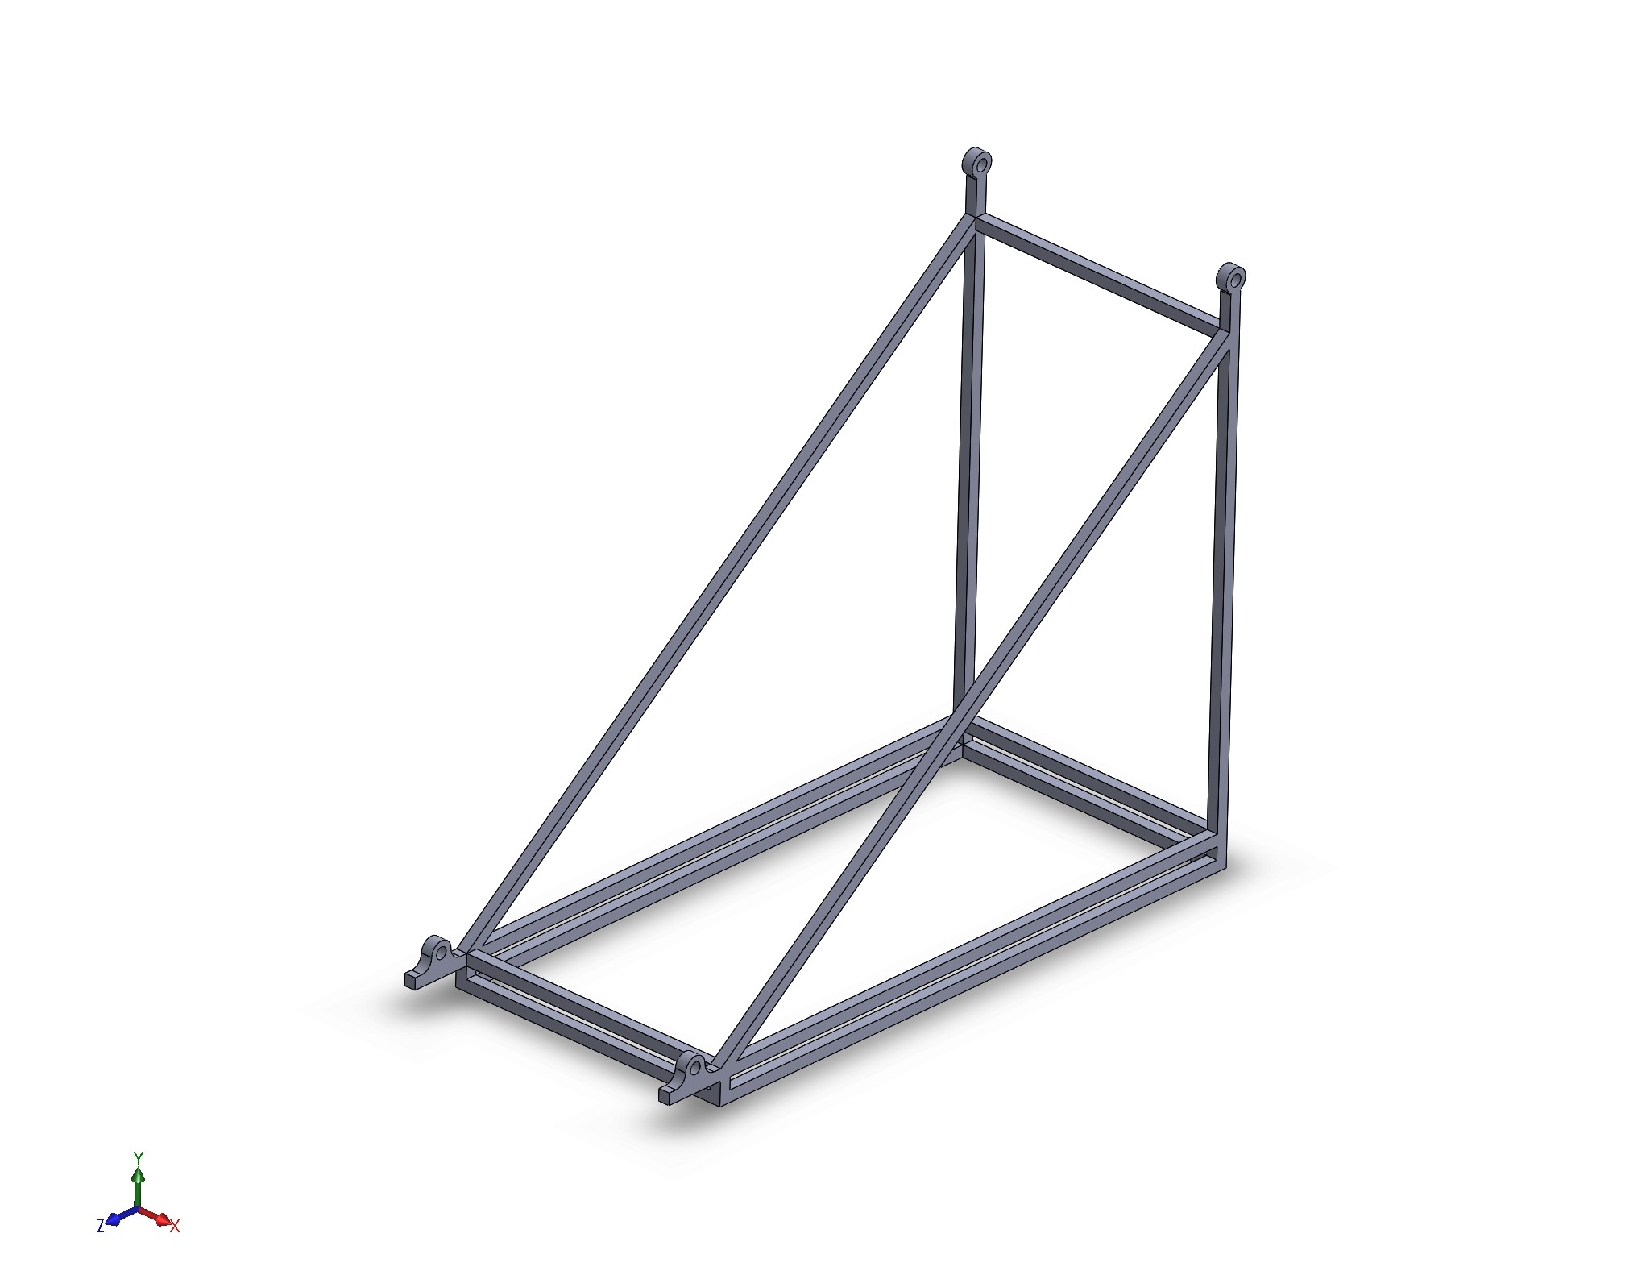
\includegraphics[scale=0.4]{MainFrame}
\caption{Main Frame}
\end{figure}


\section{Front Scraper} \label{Front Scraper}
The front scraper is the initial point of contact for the cow dung. The front scraper will be used to scrape the cow dung off the ground. The scraper must be in close proximity with the ground surface at all times, it is one of the vulnerable components of the machine, as such it must be durable enough to withstand the head on impact with the stationary cow dung.
\begin{figure}[h!]
\center
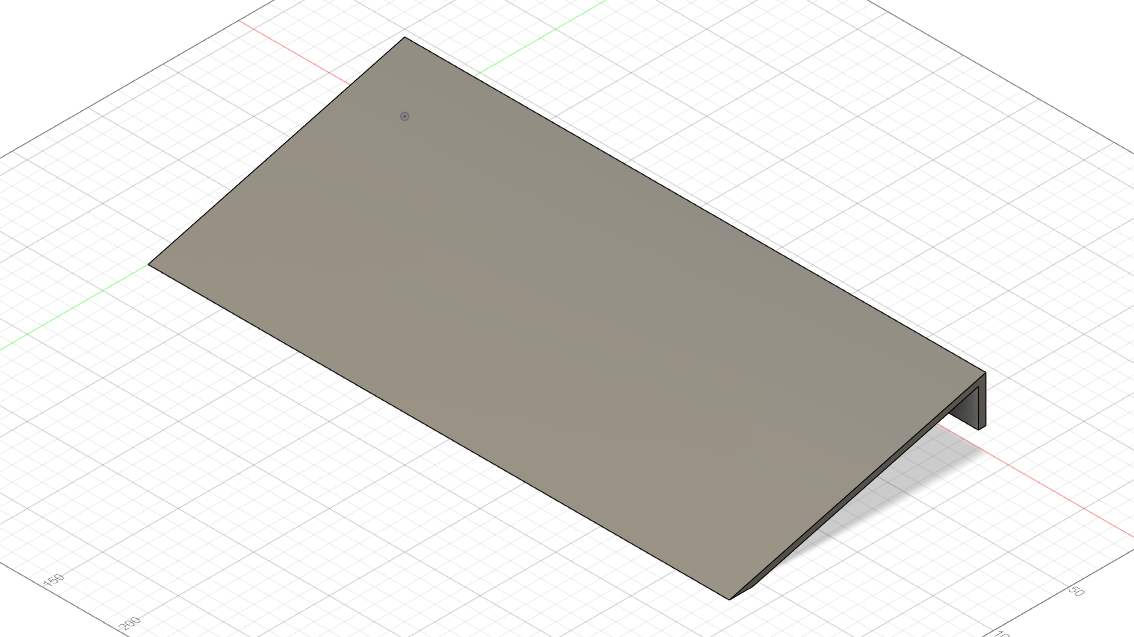
\includegraphics[scale=0.2]{Frontscraper}
\caption{Front scraper}
\end{figure}


\section{Bottom Plate} \label{Bottom Plate}
The bottom plate is one of the crucial components in evenly distributing the load of the entire machine. The bottom plate will be fixated on the main frame. It will have a small opening for the cow dung that will be collected to be dumped into the storage compartment. 
\begin{figure}[H]
\center
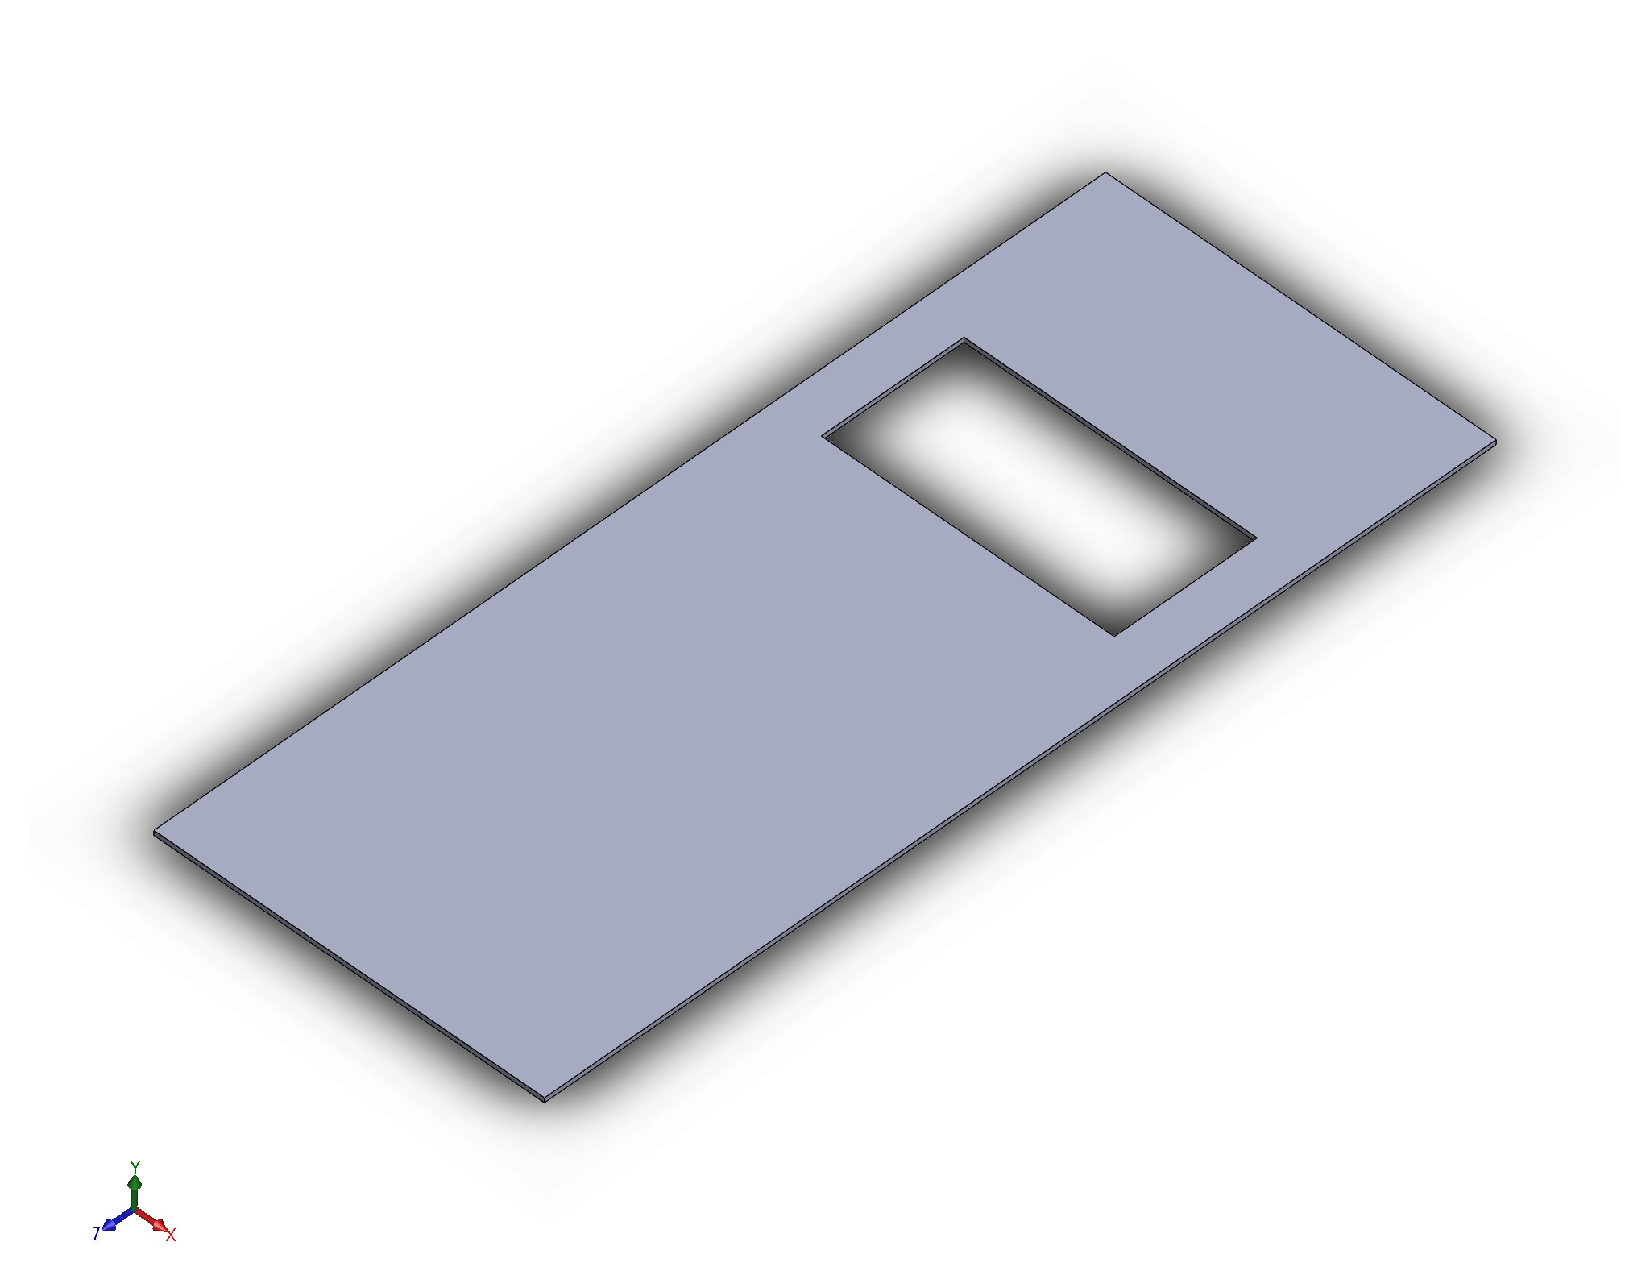
\includegraphics[scale=0.3]{BottomPlate}
\caption{Bottom Plate}
\end{figure}


\section{Blades Assembly} \label{Blades Assembly}

The blades will be in continuous motion so as to convey the cow dung from the front scraper to the storage compartment. A mount will be used to link the blades to the belt in motion. 
\begin{figure}[H]
\center
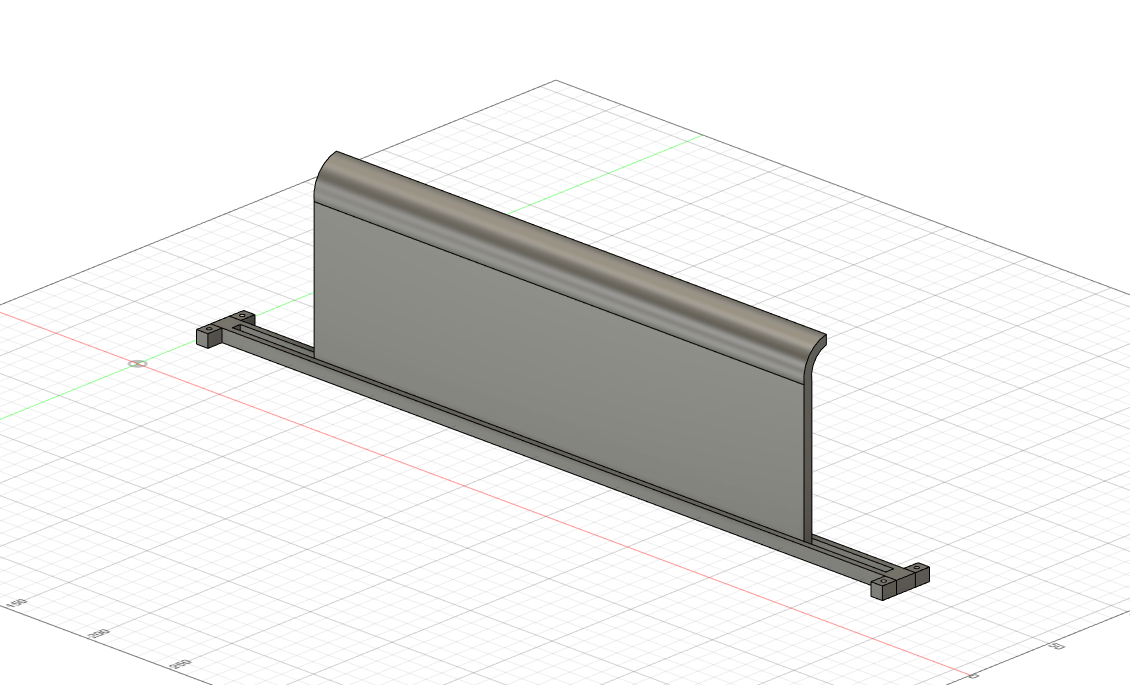
\includegraphics[scale=0.3]{BladeonMount}
\caption{Blades}
\end{figure}





\section{Shaft} \label{Shaft}
A drive shaft, driving shaft, propeller shaft is a mechanical component for transmitting torque and rotation usually used to connect other components of a drive train that cannot be connected because of distance or the need to allow for relative movement between them.




\section{Freewheel} \label{Freewheel}
 
In mechanical or automotive engineering, a freewheel or overrunning clutch is a device in a transmission that disengages the driveshaft from the driven shaft when the driven shaft rotates faster than the driveshaft. This is needed to ensure the belt assembly has it's motion constrained in one particular direction.
\begin{figure}[h!]
\center
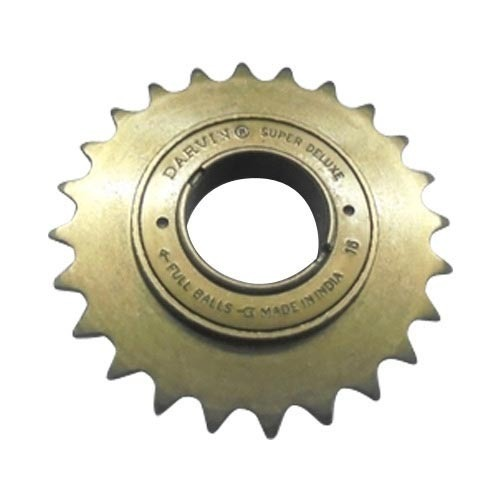
\includegraphics[scale=0.5]{24tfreewheelgear}
\caption{Freewheel}
\end{figure}


\section{Bearing
} \label{Bearing}
A bearing is a machine element that constrains relative motion between moving parts to only the desired motion. The design of the bearing may, for example, provide for free linear movement of the moving part or for free rotation around a fixed axis; or, it may prevent a motion by controlling the vectors of normal forces that bear on the moving parts.


\section{Sprocket} \label{Sprocket}
It is a profiled wheel with teeth or cogs that mesh with a chain, track or other perforated or indented material. The name sprocket applies generally to any wheel upon which are radial projections that engage a chain passing over it. It is distinguished from a gear in that sprockets are never meshed together directly, and differs from a pulley in that sprockets are never meshed together directly, and differs from a pulley in that sprockets have teeth while pulleys are smooth.
\begin{figure}[h!]
\center
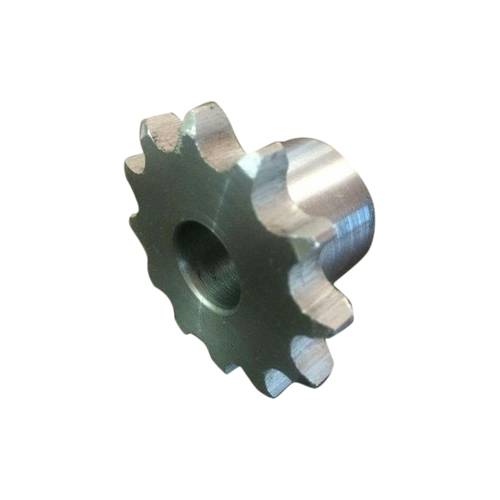
\includegraphics[scale=0.3]{12tsproket}
\caption{Sprocket}
\end{figure}


\section{Chain} \label{Chain}
Chain drive is a way of transmitting mechanical power from one place to another. It is often used to convey power to the wheels of a vehicle, particularly bicycles and motorcycles. It is also used in a wide variety of machines besides vehicles.

\begin{figure}[H]
    \centering
    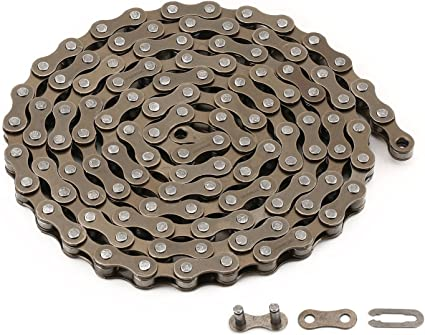
\includegraphics[scale=0.5]{chains.jpg}
    \caption{Chain}
    \label{fig:Chain}
\end{figure}

\section{Tyres} \label{Tyres}
Tyres are designed to support the weight of the machine, transmit torque and traction, and maintain and change the direction of travel. 

\begin{figure}[H]
  \centering
    \begin{minipage}{0.40\textwidth}
    \centering
      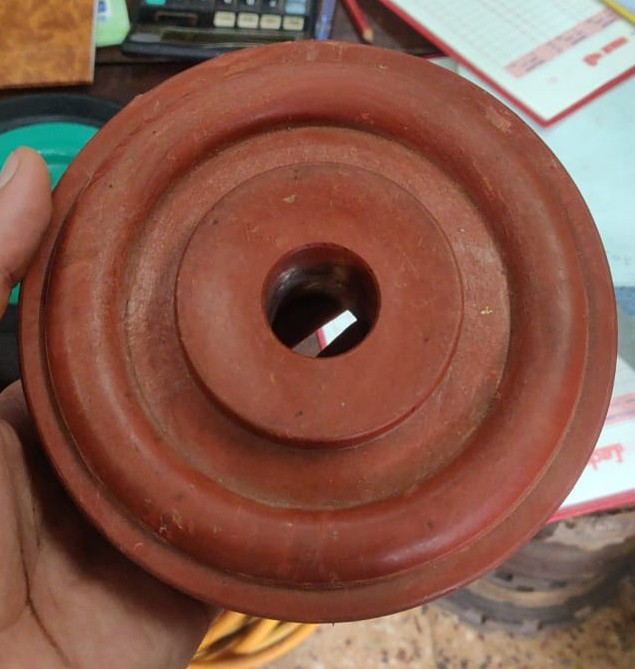
\includegraphics[width=1\textwidth]{Rubber Tyre.jpg}
      \caption{Rubber Tyre}
      \label{fig:Rubber Tyre}
    \end{minipage}
    \begin{minipage}{0.51\textwidth}
    \centering
      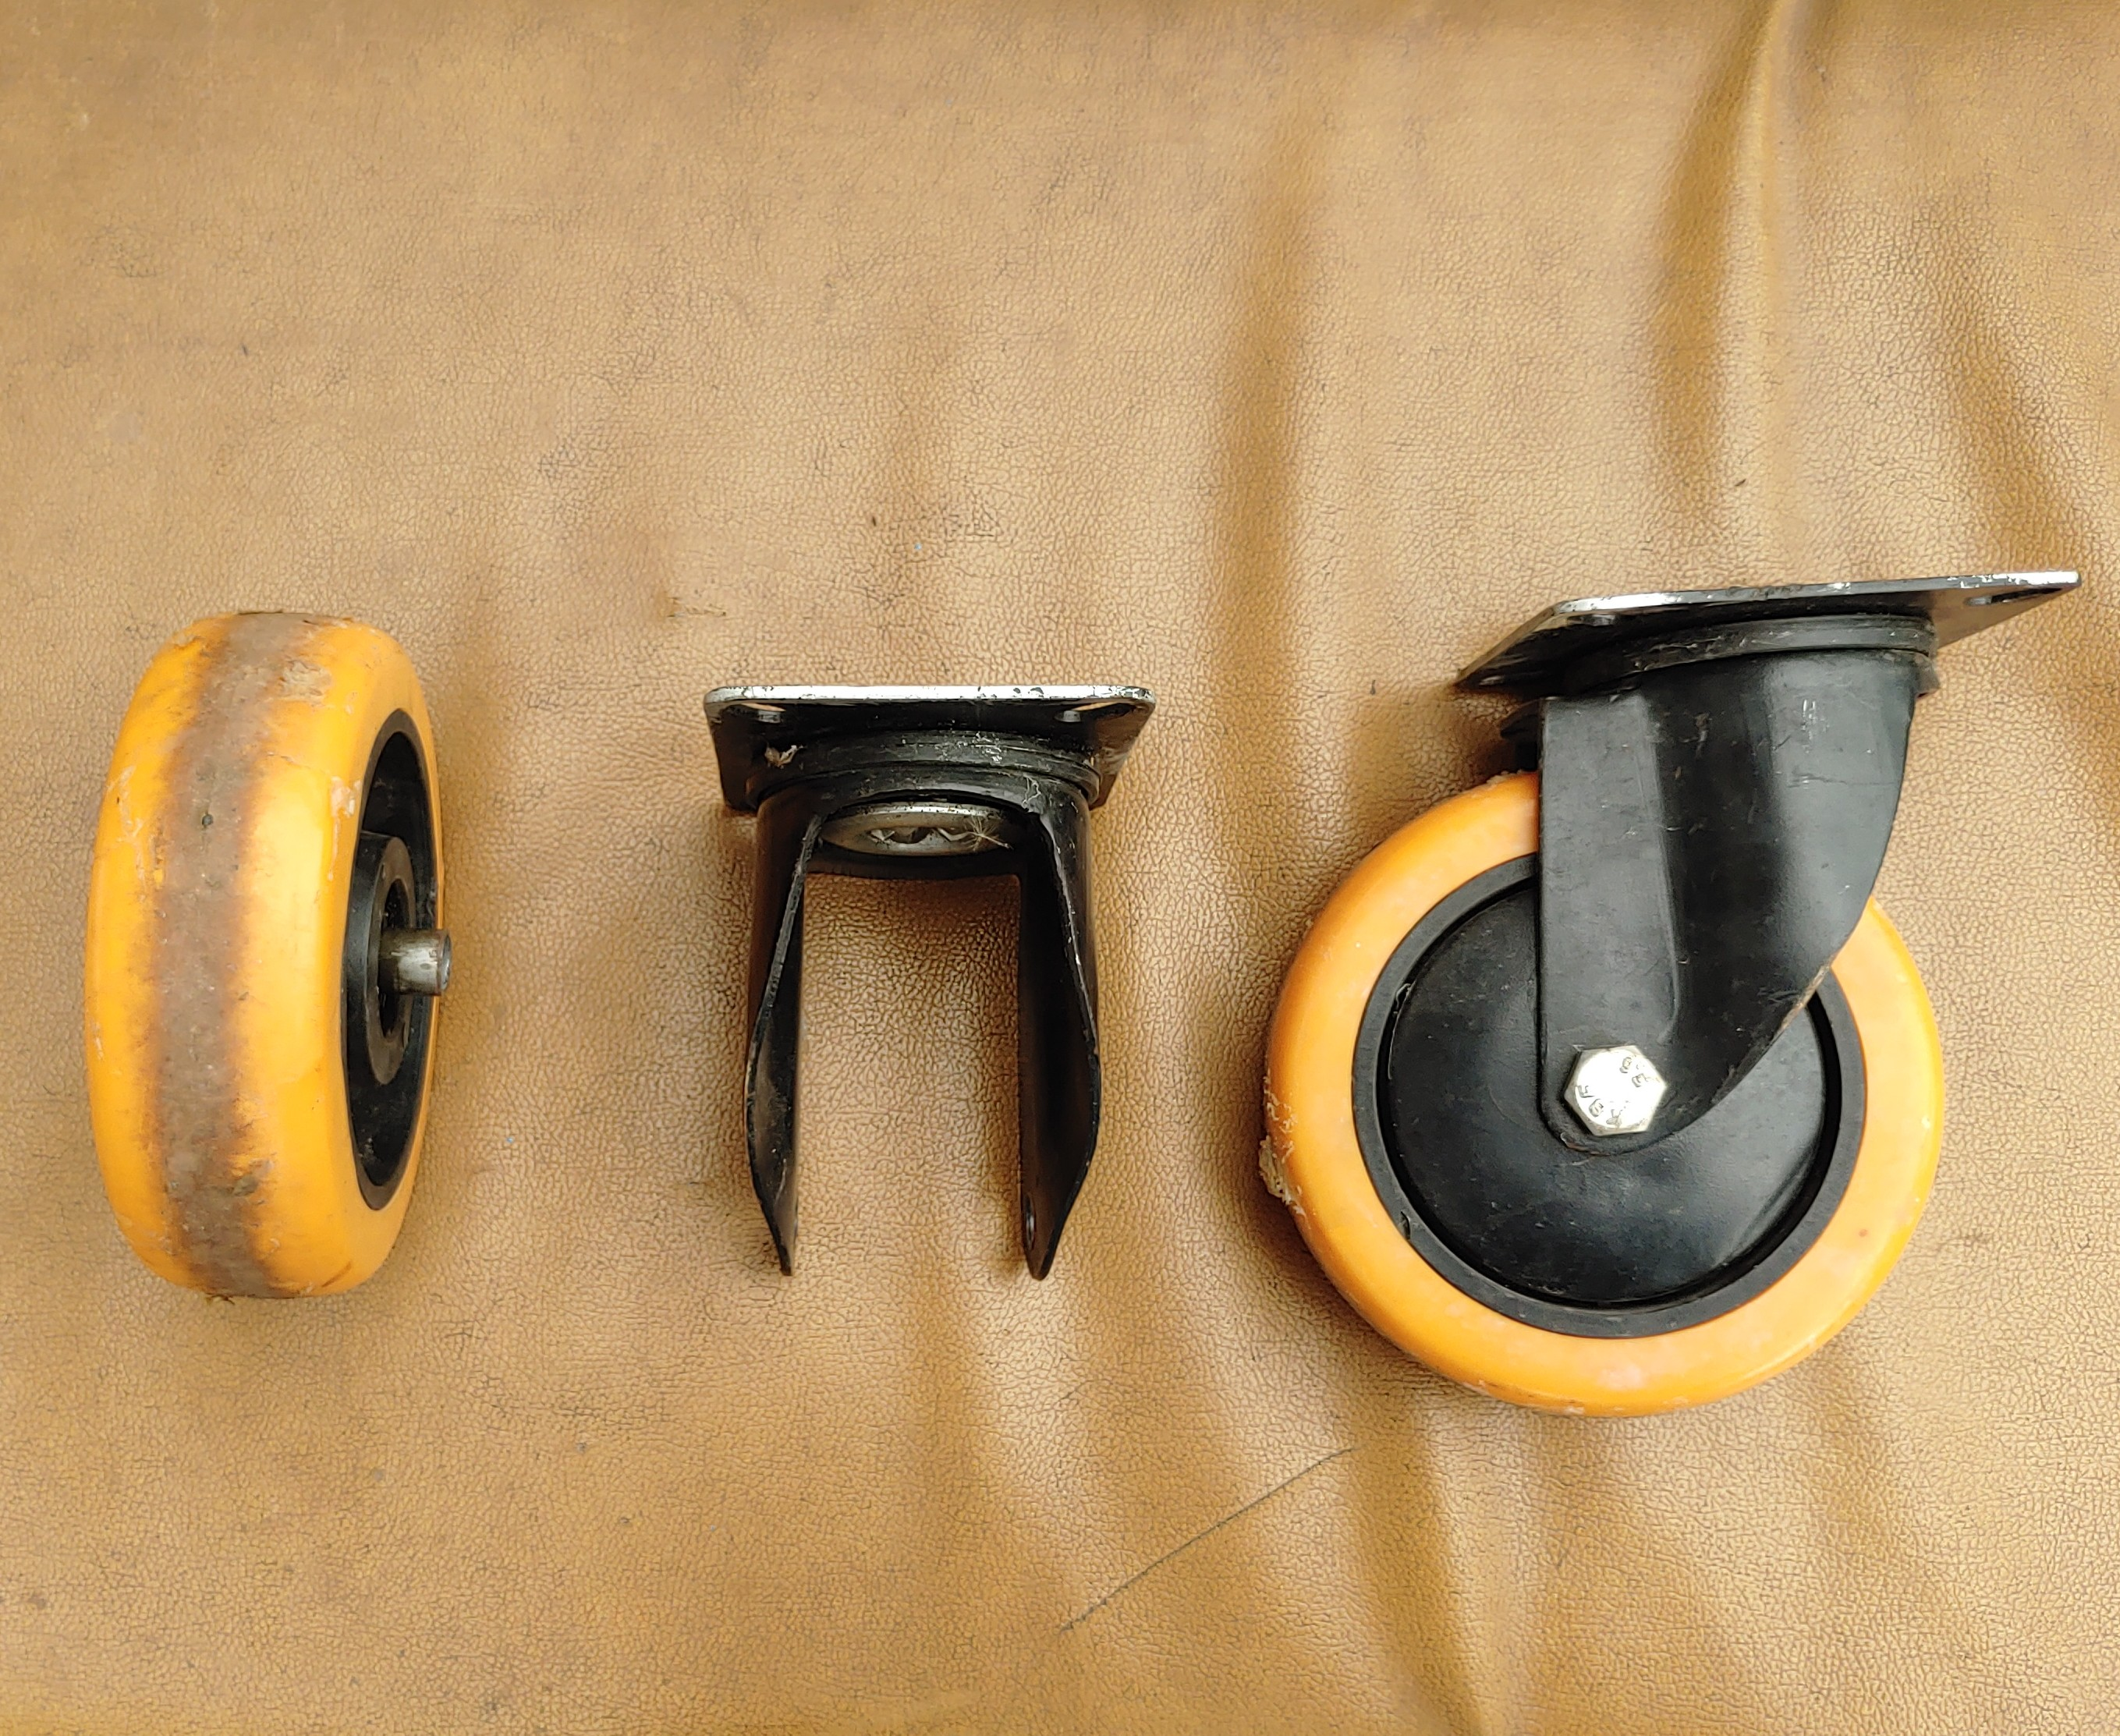
\includegraphics[width=1\textwidth]{Omnidirectional Wheel.jpg}
      \caption{Omnidirectional Tyre}
      \label{fig:Omnidirectional Tyre}
    \end{minipage}
\end{figure}







